\chapter{Logische Programmierung (Prolog)}
Das Programmierparadigma von Prolog ist \textbf{deklarativ-logisch}. Prolog ist ein Akronym für PROgrammation en LOGique. Wir beschreiben mit Logik WAS wir wollen und nicht WIE wir es berechnen. Die wichtigsten Mechanismen in Prolog sind \textbf{Matching} und \textbf{automatisches Backtracking}. Zentral ist die \textbf{Wissensdatenbank}, worin alle \textbf{Fakten \& Regeln} stecken. Die Wissensdatenbank kann angefragt werden, wobei Prolog darauf entsprechend antwortet.

\begin{figure}[h!]
\centering
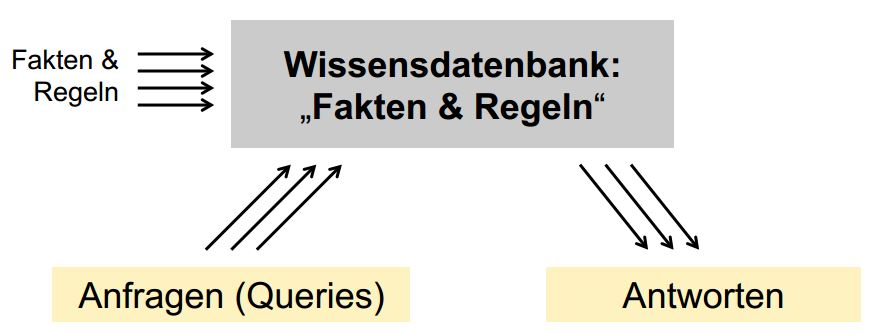
\includegraphics[width=0.7\linewidth]{fig/prolog-funktionsweise}
\caption{Funktionsweise Prolog}
\label{fig:funktionsweise-prolog}
\end{figure}

\begin{lstlisting}[caption=Wissensdatebank mit nur Fakten]
% In folgender Wissensdatenbank sind drei Fakten enthalten. Bigger definiert, dass das erste Elemente grösser als das zweite Element ist.
bigger(elephant, horse).
bigger(horse, dog).
bigger(horse, sheep).
\end{lstlisting}

\begin{lstlisting}[caption=Anfrage 1]
% Gegen die Wissensdatenbank kann eine Anfrage gemacht werden. Prolog prüft ob es für die Anfrage einen Match gibt. Jedoch existiert aber keine Match dafür. Nirgends ist definiert, dass ein Hund grösser als ein Elefant ist.
?- bigger(dog, elephant).
false.
\end{lstlisting}

\begin{lstlisting}[caption=Anfrage 2]
% Für folgende Anfrage ist ein Match vorhanden. Fakt 1 in der Wissensdatenbank matcht die Anfrage.
?- bigger(elephant, horse).
true.
\end{lstlisting}

\newpage
\begin{lstlisting}[caption=Anfrage mit Variable]
% Bei Anfragen können auch Variabeln definiert werden. Alle gross geschriebenen Wörter sind Variabeln. Prolog sucht nun nach allen Matches, welche als erstes Element horse haben. Als Resultat werden alle möglichen X Werte geliefert. (Prolog liefert immer nur ein Resultat - möchte man weitere Resultate ansehen, muss Semikolon gedrückt und um die Abfrage zu beenden den Punkt Operator wählen.)
?- bigger(horse, X).
X = dog ;
X = sheep ;
false.
\end{lstlisting}

\begin{lstlisting}[caption=Transitive Hülle von \emph{bigger/2}]
% Wir wissen implizit, dass der Elefant grösser ist als der Hund. Da der Elefant grösser als das Pferd ist und das Pferd grösser als der Hund. Aber eine Anfrage ob der Elefant nun grösser als der Hund ist, würde false liefern. Es müssen Regeln definiert werden, welche diese Beziehung unter den Fakten abbilden. Wir definieren für bigger/2 eine transitive Hülle.
is_bigger(X, Y) :- bigger(X, Y).
is_bigger(X, Y) :- bigger(X, Z), is_bigger(Z, Y).
\end{lstlisting}

\begin{lstlisting}[caption=Transitive Anfrage]
?- is_bigger(elephant, dog).
true.
\end{lstlisting}

\begin{lstlisting}[caption=Transitive Anfrage mit Variabeln]
% Selbstverständlich können nun auch Anfragen mit Variabeln über die transitive Hülle durchgeführt werden.
?- is_bigger(X, dog).
X = horse ;
X = elephant ;
false.
\end{lstlisting}

\begin{lstlisting}[caption=Verknüpfen von Anfragen]
% Es können auch verknüpfte Anfragen (UND) ausgeführt werden.
?- is_bigger(elephant, X), is_bigger(X, dog).
X = horse ;
false.
\end{lstlisting}

\begin{lstlisting}[caption=Regel umkehren]
% Eine is_smaller/2-Regel ist schnell implementiert.
is_smaller(X, Y) :- is_bigger(Y, X).
\end{lstlisting}

\newpage
\section{Syntax}
In Prolog gibt es verschiedene Typen von Termen.

\begin{figure}[h!]
\centering
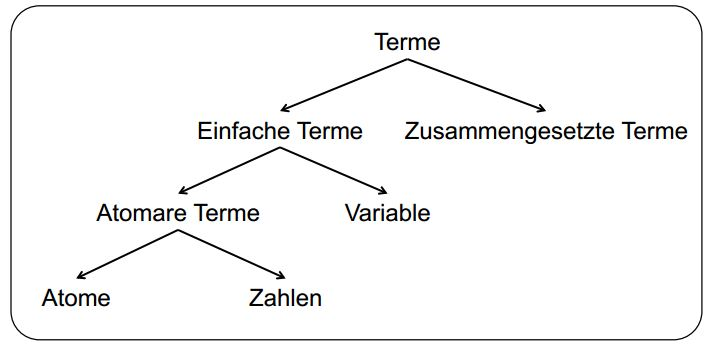
\includegraphics[width=0.5\linewidth]{fig/prolog-terme}
\caption{Übersicht Terme in Prolog}
\label{fig:prolog-terme}
\end{figure}

\begin{description}
	\item[Zahlen] (numbers) Gelten auch als atomare Terme (atomic Terms): 123, 4657.8, -9
	
	\item[Atome] (atoms) Beginnen mit Kleinbuchstaben oder sind in einfachen Anführungszeichen eingeschlossen. Gelten auch als atomare Terme (atomic Terms): elephant, 'mein text'
	
		\item[Zusammengesetzte Terme] (compound terms) Bestehen aus dem Funktor (functor) und Argumenten. Der Funktor ist ein Atom (is\_bigger) und die Argumente sind Terme: is\_bigger(horse, X)
	
	\item[Variablen] (variables) Beginnen mit Grossbuchstaben oder einem Unterstrich: X, Elephant, \_, \_elephant
	
	\item[Anonyme Variable] Die Variable \_ (Unterstrich) heisst \textbf{anonyme Variable}. Diese dient als Platzhalter, dessen Wert nicht interessiert. Jedes auftreten repräsentiert eine neue Variable. 
	
	\begin{lstlisting}[caption=Anfrage mit anonymer Variable]
	?- is_bigger(_, horse).
	true .
	\end{lstlisting}
		
	\item[Grundterme] (ground terms) Terme ohne Variablen. Diese sind als sogenannte Fakten bekannt: bigger(you, me) oder write('hello').
	
	\item[Prädikate] (predicates) Atome und zusammengesetzte Terme. Treten sie als Atome auf sind es Fakten (bigger) sonst sind es Regeln (is\_bigger(X, Y) :- bigger(X, Y).
	
	\item[Stelligkeit] (arity) Die Stelligkeit eines Prädikats zeigt auf wie viele Argumente das Prädikat entgegennimmt. Die Stelligkeit wird am Schluss des Prädikats angegeben: is\_bigger/2
	
	\item[Anfragen] (queries) sind Prädikate oder Sequenzen von Prädikaten gefolgt von einem Punkt. Der Punkt veranlasst Prolog zu antworten.
	
	\item[Klauseln] (clauses) sind Fakten und Regeln (zusammengesetzte Terme).
	
	\item[Prozedur] (procedure) Alle Klauseln zum gleichen Prädikat (d.h alle Relationen mit gleichem Name (Funktor) \& Stelligkeit).
	
	\item[Prolog-Programm] Liste aller Klauseln.
	
	\item[Fakten] (facts) Typischerweise Grundterme.
	
	\item[Regeln] (rules) Bestehen aus einem Kopf (head) und einem Hauptteil (body), welche durch :- getrennt sind. Der Kopf einer Regel ist wahr, wenn alle Ziele (Prädikate) im Hauptteil als wahr bewiesen werden. Ziele werden durch Komma getrennt, welches eine UND-Verknüpfung darstellt (Konjunktion).
	
	\begin{lstlisting}[caption=Regel]
	grandfather(X, Y) :- % head
	father(X, Z), % body, goal 1
	parent(Z, Y). % body, goal 2
	\end{lstlisting}
	
	\emph{Prolog nutzt ein spezielles System von logischen Formeln, die sogenannten \textbf{Hornklauseln}: ((p1 AND p2 AND ... AND pn) -> q) }. Sind alle Bedingungen auf der linken Seite erfüllt, lässt sich die rechte Seite daraus ableiten (Konjunktion und Implikation).
\end{description}

\section{Matching}
Wenn Anfragen an das Prolog-System gestellt werden, führt Prolog eine Beweissuche mittels Backtracking und Matching durch. Zwei Terme matchen, wenn sie identisch sind oder wenn sie durch ersetzen von Variabeln durch andere Terme identisch gemacht werden können. Mittels dem Gleichheits-Prädikat =/2 kann abgefragt werden, ob zwei Terme matchen.

\begin{lstlisting}[caption=Gleichheits-Prädikat]
?- eat(tom, burger) = eat(X, burger).
X = tom.
?- eat(tom, burger) = eat(X, potato).
false.
\end{lstlisting}

\begin{lstlisting}[caption=Gleichheits-Prädikat auf Atomen]
% Atome matchen, wenn sie genau gleich sind.
?- =(tom, tom). % Predefined predicate =/2
true.
?- tom = tom. % other style: =/2 as infix operator
true.
?- 'Tom' = tom. % Watch out: case sensitive!
false.
?- 'tom' = tom. % =/2 ignores single quotes
true.
\end{lstlisting}

\begin{lstlisting}[caption=Gleichheits-Prädikat auf Variabeln und Termen]
% Falls ein Term eine Variable ist, dann matchen beide Terme und die Variable wird dem Wert des zweiten Terms instanziiert.
?- pia = X.
X = pia.
?- sing(pia) = X.
X = sing(pia).
?- X = Y.
X = Y.
?- X = Y, X = pia.
X = Y, Y = pia.
?- X = Y, X = pia, Y = tom.
false.
\end{lstlisting}

\begin{lstlisting}[caption=Gleichheits-Prädikat auf zusammengesetzten Termen]
% Matchen wenn gleicher Funktor, gleiche Stelligkeit und alle korrespondierende Argumente matchen.
?- meet(drink(pia), eat(X)) = meet(Y, eat(tom)).
X = tom,
Y = drink(pia).
?- meet(X, X) = meet(drink(pia), tom).
false.
?- meet(pia, tom) = meet(Y).
false.
\end{lstlisting}

\begin{lstlisting}[caption=Unendliche Terme]
% Was passiert da?
?- f(A)=A.
% Gemäss Matching-Regeln müsste das Resultate so aussehen (unendlich):
A = f(f(f(f(f(f(f(f(f(f(f(...
% Da in Prolog standardmässig kein occurs-check gemacht wird, kommt folgendes:
A = f(A).
\end{lstlisting}

\emph{In der Logik ist die Unifikation ein bekanntes Verfahren zur Verinheitlichung von Ausdrücken. Ähnlich wie bei Prolog das Matching. Der Unterschied besteht darin, dass beim Matching kein occurs-check gemacht wird. Falls eine Variable mit einem Term vereinheitlicht wird, wird zuerst geprüft, ob diese Variable in diesem Term vorkommt. Aus Effizienzgründen wird das in Prolog nicht gemacht. Es kann jedoch explizit ausgeführt werden unify\_with\_occurs\_check(+Term1, +Term2) was beim obigen Beispiel zu false evaluieren würde.}

\section{Beweissuche und Suchbäume}
Das Prolog-System versucht die Anfrage zu beweisen. Dazu versucht es die Fakten und Regeln in der Wissensdatenbank zu matchen. Dabei verwendet es ein Backtracking-Algorithmus, welches eine Tiefensuche darstellt. Falls die Anfrage aufgelöst werden kann, liefert es true oder gegebenenfalls die Matchings zurück. Ansonsten false. Die Anordnung der Regel und Fakten in der Wissensdatenbank beeinflusst wie schnell Prolog zu einer Lösung kommt.

\begin{itemize}
	\item Suche in der Wissensdatenbank von oben nach unten
	\item Abarbeitung der Abfrage-Klauseln von links nach rechts
	\item Backtracking zur Erholung von „schlechten“ Pfaden
\end{itemize}

\begin{figure}[h!]
\centering
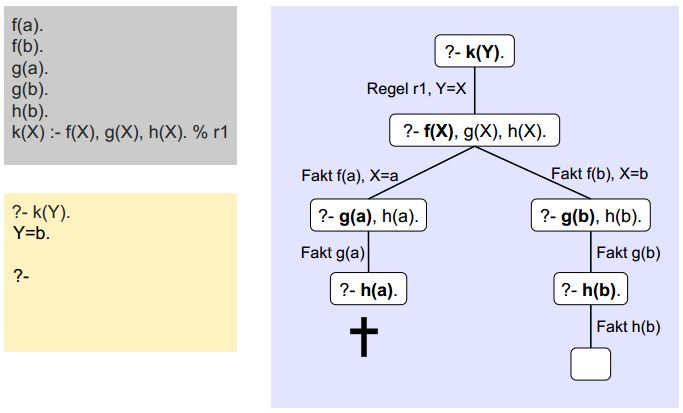
\includegraphics[width=0.47\linewidth]{fig/prolog-beweissuche-suchbaueme}
\caption{Prolog: Beweissuche und Suchbäume}
\label{fig:prolog-beweissuche-suchbaueme}
\end{figure}

\section{Deklarative vs. Prozedurale Bedeutung}
Grundsätzlich reicht es in Prolog die deklarative Bedeutung (WAS - Problem-Beschreibung - deklarativ-logisch) anzugeben und es muss nicht die prozedurale Bedeutung (WIE - Beschreibung der Problemlösung - imperativ) definiert werden. Der deklarative Weg reicht leider nicht immer. Aus Ausführungseffizienzgründen gibt es in Prolog prozedurale Konstrukte wie Endrekursion, Assertions, Cut-Operator \& Negation. Conclusion: Wenn das Problem modelliert ist, ist es (grundsätzlich) gelöst. Einzige Einschränkung ist die Effizienz, welches in der prozeduralen Programmierung gesteuert werden kann. Oft es auch nicht einfach das Problem zu modellieren. Übung macht den Meister wie bei guter OO-Modellierung.

\section{Typische Prolog-Poblemstellungen}
Mit Prolog lassen sich auf nette Art und Weise folgende Problemstellungen lösen: Kreuzworträtsel, Färben von Karten, Zahlenrätsel, Sudoku, Spracherkennung, Expertensysteme u.v.a.m.

\subsection{Kreuzworträtsel}
\begin{enumerate}
	\item Jedes leere Feld muss mit einem Identifier markiert werden, welcher als Platzhalter für einen Buchstaben dient.
	\item  In der Wissensdatenbank müssen alle möglichen Wörter definiert werden.
	\item Regeln für alle Wörter aus dem Kreuzworträtsel definieren.
	\item Anfrage formulieren und ausführen.
\end{enumerate}

\begin{figure}[h!]
\centering
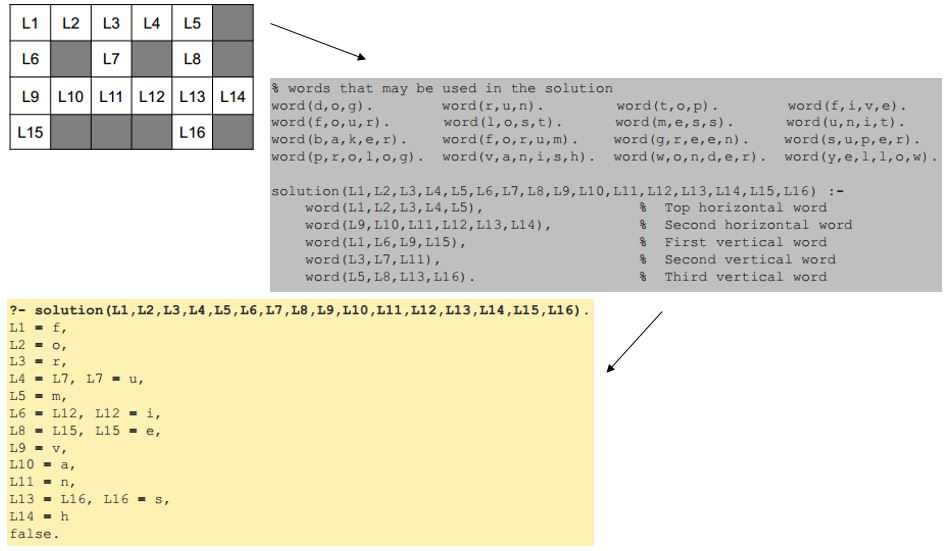
\includegraphics[width=1\linewidth]{fig/prolog-kreuzwortraetsel}
\caption{Prolog: Kreuzworträtsel lösen}
\label{fig:prolog-kreuzwortraetsel}
\end{figure}

\subsection{Karten färben}
Es liegt eine fixe Anzahl an unterschiedlichen Farben vor. Nun sollen die Länder auf einer Karte eingefärbt werden, wobei angrenzende Länder unterschiedlich gefärbt sein sollen. 
\begin{enumerate}
	\item Definition von Prädikaten, welche Farben nebeneinander sein dürfen.
	\item Definition von Ländern, welche nebeneinander liegen. Da diese alle um die gleiche Zeit erfüllt sein müssen, werden diese als Konjunktion definiert.
\end{enumerate}

\begin{figure}[h!]
\centering
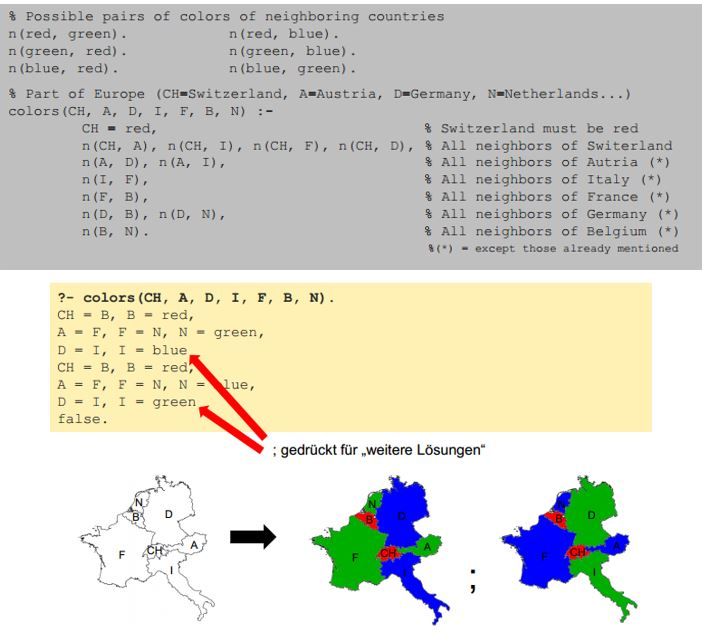
\includegraphics[width=1\linewidth]{fig/prolog-karten-faerben}
\caption{Prolog: Karten färben}
\label{fig:prolog-karten-faerben}
\end{figure}

\newpage
\section{Operatoren und Prädikate}
Operatoren und Prädikate sind dasselbe. Es sind einfach zwei unterschiedliche Schreibweisen. Grundsätzlich gibt es nur Prädikate, welche aber auch als Operatoren verwendet werden könne.

\begin{lstlisting}[caption=Prädikat >/2]
?- 3 > 7. % infix operator style for predicate >/2
false.
?- >(3, 7). % >/2 predicate, "regular style"
false.
\end{lstlisting}

Mittels dem Prädikat \emph{op/3} op(+Precedence, +Type, :Name) können Prädikate als Operatoren deklariert werden.

\begin{lstlisting}[caption=is\_bigger/2 als Operator]
?- op(1150, xfx, is_bigger). % declare new operation
true.
?- elephant is_bigger dog. % use our new operation
true.
\end{lstlisting}

Die \textbf{Präzedenz} (Operatorrangfolge) von einem Operator definiert, wie stark ein Operator seine Operanden bindet. Eine tiefere Präzedenz bedeutet eine stärkere Bindung. Dadurch wird definiert, wann welcher Operator auf seine Operanden angewendet wird. In SWI-Prolog wird dieser Wert zwischen 1 und 1200 angegeben. Der Haupt-Funktor von einem Term ist der Operator mit der höchsten Präzedenz. Der \textbf{Operator-Typ} definiert die relative Reihenfolge von Operator f und Operanden x und y. Es gibt drei Typen:

\begin{description}
	\item[Infix] xfx, xfy, yfx. Operator ist zwischen den beiden Operanden.
	\item[Präfix] fx, fy. Operator f ist vor dem Operand.
	\item[Postfix] xf, yf. Operator f ist nach dem Operand.	
\end{description}

Mit x und y wird die Präzedenz der Operanden einer Operation f festgelegt. X repräsentiert einen Operanden, dessen Präzedenz strickt kleiner ist als die Präzedenz vom Operator f. Y repräsentiert einen Operanden, dessen Präzedenz kleiner oder gleich derjenige vom Operator f ist. Dies dient schlussendlich dazu, dass auch folgendes korrekt ausgewertet wird: \emph{1 - 2 - 3 }. 

\begin{figure}[h!]
\centering
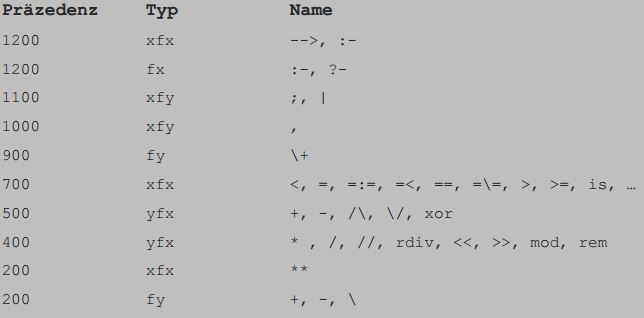
\includegraphics[width=0.7\linewidth]{fig/prolog-operatoren}
\caption{Prolog: Operatoren}
\label{fig:prolog-operatoren}
\end{figure}

\newpage
In der API-Dokumentation von Prolog werden folgende Zeichen eingesetzt:
\begin{description}
	\item[-] Operand sollte ungebunden (d.h. nicht instanziiert) sein. Also eine Variable (Wert wird durch Prädikat zugewiesen).
	\item[+] Operand sollte gebunden (d.h. instanziiert) sein. Also eine Zahl, ein Atom oder ein gebundener zusammengesetzter Term (Term wird vom Prädikat gebraucht).
	\item[?] Operand kann gebunden oder ungebunden sein.
\end{description}

\subsection{Arithmetische Operatoren}
+ Addition, - Subtraktion, * Multiplikation, / Division, ** Potenz, // Ganzzahldivision, mod Modulo (Rest bei Ganzzahldivision). Wenn versucht wird \emph{X = 1 + 2} zu berechnen, gelingt dies nicht, da der Gleich-Operator dem Matching dient. Dafür muss der \emph{is/2}-Operator verwendet werden \emph{(X is 1 + 2)}. Der Ausdruck \emph{(8 is X)} würde ein Runtime-Fehler geben. Die Definition von dem \emph{is/2-Operator} ist folgende: \emph{-Number is +Expr}.

\begin{lstlisting}[caption=Arithmetische Terme]
?- D is 5/2. % division
D = 2.5.
?- I is 5//2. % integer division
I = 2.
?- Z is 5 mod 2. % modulo (remainder of integer div.)
Z = 1.
?- P is 2 ** 4. % power
P = 16.
?- C is cos(0). % cosine
C = 1.0.
?- S is sqrt(9). % square root
S = 3.0.
\end{lstlisting}

\subsection{Vergleichsoperatoren}
> grösser als, < kleiner als, >= grösser-gleich, =< kleiner-gleich, =:= Gleichheit, =\= Ungleichheit.

\begin{lstlisting}[caption=Terme mit Vergleichen]
?- 55 > 6. % is 55 is greater than 6?
true.
?- 88 =< 77. % is 88 smaller or equal than 77?
false.
?- 1 + 2 = 2 + 1. % Attention: matching!
false. % 1+2 does not match 2+1
?- 1 + 2 =:= 2 + 1. % is 1+2 equal to 2+1?
true.
?- 44 =\= 42 + 1. % is 44 unequal to 42+1?
true.
\end{lstlisting}

\newpage
\section{Rekursion}
Prolog Prädikate können rekursiv definiert sein. Ein Prädikat ist rekursiv definiert, falls sich eine oder mehrere Regeln in ihrer Definition auf sich selber beziehen. Dies wird in Prolog häufig eingesetzt.

\begin{lstlisting}[caption=Beispiel Rekursion]
is_bigger(X, Y) :- bigger(X, Y). % simple case - Rekursionbasis
is_bigger(X, Y) :- bigger(X, Z), is_bigger(Z, Y). % general case - Rekursionsvor.
\end{lstlisting}

\begin{figure}[h!]
\centering
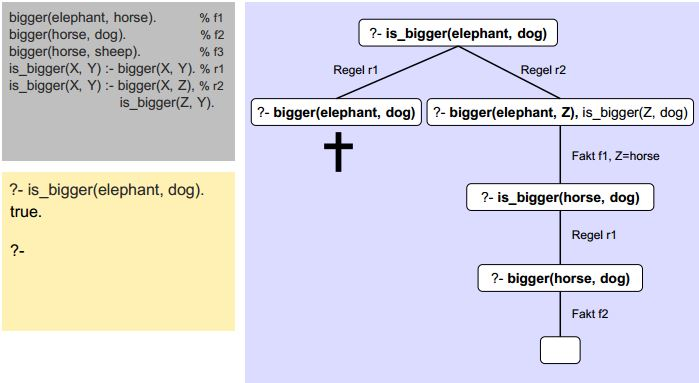
\includegraphics[width=0.7\linewidth]{fig/prolog-suchbaum-rekursion}
\caption{Prolog: Rekursions-Suchbaum}
\label{fig:prolog-suchbaum-rekursion}
\end{figure}

\begin{lstlisting}[caption=Fakultät]
fak(0, 1). 				% simple case
fak(N, F) :- 			% general case
	N > 0, 				% argument test
	N1 is N - 1, 		% evaluate N-1
	fak(N1, F1), 		% recursive call
	F is N * F1. 		% sum up

?- fak(5, X). X = 120 .
?- fak(4, 24). true.
?- fak(X, 24). ERROR: >/2: Arguments are not sufficiently instantiated
\end{lstlisting}

\begin{lstlisting}[caption=Fibonacci, label=lst:naiv-fib]
% Naive Implementierung! Optimierung mittels Endrekursion und Assertions.
fib(0, 0).
fib(1, 1).
fib(N, F) :-
	N > 1,
	N1 is N - 1,
	N2 is N - 2,
	fib(N1, F1),
	fib(N2, F2),
	F is F1 + F2.

?- fib(7, X). X = 13 .
?- fib(6, 8). true .
?- fib(X, 8). ERROR: >/2: Arguments are not sufficiently instantiated (Da brauchen wir CLP!)
\end{lstlisting}


\section{Optimierungen}
Backtracking ist grundsätzlich nicht sehr effizient. Wir können. Um dies zu entschärfen gibt es zwei bekannte Methoden: Endrekursion und Assertions.

\subsection{Optimierung durch Endrekursion}
Die Endrekursion ist auch bekannt als \emph{tail recursion}. Der Vorteil ist, dass kein Backtracking benötigt wird. Eine Endrekursion kann als Iteration ohne zusätzlichen Speicherplatz ausgeführt werden. Eine Prozedur ist endrekursiv, wenn:

\begin{itemize}
	\item Nur ein einzigen rekursiven Aufruf hat.
	\item Dieser Aufruf ist der letzte Aufruf in der letzten Klausel der Prozedur.
	\item Alle Aufrufe vor dem rekursiven Aufruf müssen deterministisch sein.
\end{itemize}

Prolog führt folgende endrekursive Prozedur als Iteration aus. Es wird viel weniger Speicherplatz benötigt. Diese Optimierung nennt sich auch \emph{last call optimization}.

\begin{lstlisting}[caption=Endrekursion: Allg. Beispiel]
p(...) :- ... 	% no recursive call in the body
p(...) :- ... 	% no recursive call in the body
...
p(...) :- ..., 	% all deterministic and
	..., 		% no recursive call until here
	p(...). 	% tail-recursive call
\end{lstlisting}

Im Listing \ref{lst:naiv-fib} ist die rekursive Berechnung alles andere als effizient. Möchte man die Fibonacci Zahl für 30 berechnen, führt dies auf herkömmlichen Rechnern zu einem \emph{ERROR: Out of local stack}. Das Problem ist, dass viele Zwischenresultate mehrmals berechnet werden müssen. Für \emph{f(6)} muss 5x \emph{f(2)} ausgewertet werden. Die Umwandlung von einem naivem Prolog-Programm in ein endrekursives ist nicht trivial! Typischerweise werden zusätzlich neue Argumente verwendet: Akkumulatoren. Diese werden verwendet um Zwischenresultate zu speichern.

\begin{lstlisting}[caption=Endrekursive Fibonnaci-Berechnung]
fib_tr(N, F) :- fib_tr(N, 0, 1, F). % call accumulator
fib_tr(0, A, _, A). 				% simple case
fib_tr(N, A, B, F) :- 				% general case
	N1 is N - 1, 					% new argument N1
	N1 >= 0, 						% avoid underflow
	Sum is A + B,					% accumulator Sum
	fib_tr(N1, B, Sum, F). 			% tail-recursisve call
\end{lstlisting}

Fazit: Falls der Speicherplatz bei einer rekursiven Prozedur kritisch wird, hilft die Umwandlung in ein endrekursive Prozedur. Diese kann als Iteration ausgeführt werden, benötigt oft weitere Argumente: Akkumulatoren.

\newpage
\subsection{Optimierung durch Assertions (Memoization)}
Die Wissensdatenbank kann nicht nur statisch sondern auch dynamisch zur Laufzeit manipuliert werden. Dies kann für Memoization (auch Caching) genutzt werden.

\begin{lstlisting}[caption=dynamic/1]
% Damit Prädikate zur Laufzeit modifiziert werden können, müssen diese mit dynamic definiert werden.
:- dynamic bigger/2.
bigger(elephant, horse).
bigger(horse, dog).
bigger(horse, sheep).
\end{lstlisting}

\begin{lstlisting}[caption=listing/1]
% Mittels listing können die Fakten und Regel zu einem Prädikat angezeigt werden.
?- listing(bigger).
:- dynamic bigger/2.
bigger(elephant, horse).
bigger(horse, dog).
bigger(horse, sheep).
\end{lstlisting}

\begin{lstlisting}[caption=asserta/1 \& assertz/1]
% Asserta fügt einen neuen Fakt an den Beginn hinzu.
?- asserta(bigger(me, you)).
true.
?- listing(bigger).
:- dynamic bigger/2.
bigger(me, you). % new fact as first rule
bigger(elephant, horse).
bigger(horse, dog).
bigger(horse, sheep)..

% Assertz fügt einen neuen Fakt an den Schluss hinzu.
?- assertz(bigger(elephant, me)).
true.
?- listing(bigger).
:- dynamic bigger/2.
bigger(me, you).
bigger(elephant, horse).
bigger(horse, dog).
bigger(horse, sheep).
bigger(elephant, me). % new fact asserted as last rule
\end{lstlisting}

\begin{lstlisting}[caption=retract/1]
% Mittels retract können Fakten/Regeln entfernt werden.
?- retract(bigger(me, you)).
true.
?- listing(bigger).
:- dynamic bigger/2.
bigger(elephant, horse).
bigger(horse, dog).
bigger(horse, sheep).
bigger(elephant, me).
\end{lstlisting}

\newpage
\begin{lstlisting}[caption=Naive Fibonnaci optimiert mit Assertions]
% Nach jeder Berechnung einer Fibonacci Zahl wird diese in die Wissensdatenbank an den Anfang (wichtig) gespeichert. Diese müssen nun nicht mehr neu berechnet werden.
:- dynamic fib_as/2.
fib_as(0, 0). 				% base case 1
fib_as(1, 1). 				% base case 2
fib_as(N, F) :- 			% general rule
	N > 1, 					% allow no negative numbers
	N1 is N-1, 
	N2 is N-2,
	fib_as(N1, F1), 		% calculate F1 = fib(N-1)
	fib_as(N2, F2), 		% calculate F2 = fib(N-2)
	F is F1+F2,
	asserta(fib_as(N, F)). 	% assert new fact
\end{lstlisting}

\section{Listen}
In Prolog gibt es Listen als Datenstrukturen. Eine Liste ist eine endliche Sequenz von Elementen. Listen werden mit eckigen Klammern dargestellt. Die Länger einer Liste ist die Anzahl darin enthaltenen Elemente. Listen-Elemente sind beliebige Terme. Die leere Liste [] ist eine spezielle Liste.

\begin{lstlisting}[caption=Listen in Prolog]
?- X = [a, b, c].
X = [a, b, c].
?- Y = [d, e, f(X), [x, y]].
Y = [d, e, f(X), [x, y]].
?- Z = [].
Z = [].
\end{lstlisting}

Die nicht-leeren Listen bestehen immer aus dem ersten Element (Kopf=head) und den restlichen Elementen (Schwanz=tail). Der Schwanz ist wiederum eine Liste. Somit sind Listen rekursiv aufgebaut.

\begin{lstlisting}[caption=Tail-Operator auf Listen]
?- [a, b, c] = [Head | Tail].
Head = a,
Tail = [b, c].

% Dies sind alles equivalente Terme.
?- L = [a | [b, c]], L = [a, b | [c]], L = [a, b, c | []].
L = [a, b, c].

% Hier interessiert nur zweites und drittes Element.
?- [_, X2, X3 | _] = [a, b, c, d, e, f].
X2 = b,
X3 = c.
\end{lstlisting}

\newpage
\subsection{Listenzugehörigkeit}
Ist X ein Element der Liste L? X kommt in der Liste vor, wenn X gleich Kopf der Liste ist oder wenn es im Schwanz der Liste vorkommt. 

\begin{lstlisting}[caption=Listenzugehörigkeit]
mem(X, [X | _]). 					% tail doesnt matter
mem(X, [_| Tail]) :- mem(X, Tail). 	% head doesnt matter

% Anmerkung: Wenn auf der linken Seite Variabeln definiert werden, welche auf der rechten Seite nicht verwendet werden, dann kommt es zur Warnung: Singleton Variables.

?- mem(b, [a, b, c]).
true.

?- mem(d, [a, b, c]) .
false.

?- mem([b, c], [a, [b, c]]).
true.

?- mem(X, [a, b, c]).
X = a;
X = b;
X = c;
false.

% Generiert unendlich lange Lösungslisten...
?- mem(a, L), mem(b, L), mem(c, L). % which list L contains a, b, & c?
L = [a, b, c|_G2239];
L = [a, b, _G2238, c|_G2242];
L = [a, b, _G2238, _G2241, c|_G2245];
...

% So wäre Permutation möglich. Die Länge der Liste beschränken!
?- L = [_, _, _], mem(a, L), mem(b, L), mem(c, L).
L = [a, b, c];
L = [a, c, b];
L = [b, a, c];
L = [c, a, b];
L = [b, c, a];
L = [c, b, a];
false.

% P.S. In Prolog gibt es bereits das Prädikat member/2.
\end{lstlisting}

\newpage
\subsection{Listenkonkatenation}
Wir wollen wissen, ob Liste L1 und Liste L2 zusammenhängt Liste L3 ergeben. Einfacher Fall: Wenn die L1 eine leere Liste ist, dann muss L2 und L3 gleich sein. Falls die erste Liste nicht leer ist, hat diese einen Kopf und Schwanz [X, L1]. Die Konkenation muss den gleichen Kopf haben, also [X, L3].

\begin{lstlisting}[caption=Listenkonkatenation]
conc([], L, L).
conc([X | L1], L2, [X | L3]) :- conc(L1, L2, L3).

% Zwei Listen konkatenieren
?- conc([a, b], [c, d], L).
L = [a, b, c, d].
?- conc([a, b], [c], [a, b, c, d]) .
false.
?- conc([a, [b, c], d], [a, [], b], L).
L = [a, [b, c], d, a, [], b].

% Zerlegung einer Liste in alle möglichen Teillisten
?- conc(L1, L2, [a, b, c]).
L1 = [],
L2 = [a, b, c];
L1 = [a],
L2 = [b, c];
L1 = [a, b],
L2 = [c];
L1 = [a, b, c],
L2 = [];
false.
\end{lstlisting}

\section{Negation von Prädikaten}

In Prolog kann eine Negation entweder mit einem Cut-Operator (\verb|!/0|) kombiniert mit \verb|fail/0| oder mit \verb|not/1| ausgedrückt werden. Als Beispiel verwenden folgende Aussage \textit{Mary mag alle Tiere ausser Schlangen}. Listing \ref{lst:negation} zeigt das obengennante Beispiel.

\begin{lstlisting}[caption=Negation, label=lst:negation]
% Wenn X eine Schlange unterbreche Backtracking und Regel ist falsch
likes(mary, X) :- snake(X), !, fail.
% Mit not/1
likes(mary, X) :- animal(X), not(snake(X)).
% Mary mag alle Tiere
likes(mary, X) :- animal(X).
\end{lstlisting}

Für \verb|not/1| gibt es noch eine alternative Syntax \verb|\+/1|, die aber die gleiche Funktion hat. \verb|not/1| ist in Prolog als \textit{schwache Negation} (negation as failure) definiert. Schwache Negation basiert auf der Closed-World-Assumption (CWA) und nicht auf der Negation in der mathematischen Logik. In Prolog wird angenommen, dass jedes Programm alles Wahre über die Welt beschreibt. Deshalb wird alles was nicht im Programm beschrieben ist als falsch angenommen. Deshalb wird die Negation von Dingen, die das Programm nicht weiss immer als wahr angenommen (schwache Negation - CWA). Listing \ref{lst:cwa} zeigt das Prolog findet die Welt ist nicht rund, obwohl sie dass eigentlich ist. Dadurch können in Prolog komische Resultate entstehen.

\begin{lstlisting}[caption=CWA, label=lst:cwa]
round(ball)

?- round(ball).
true. % as expected

?- round(earth).
false. % caused by the CWA

?- not(round(earth)).
true. % caused by negation as failure
\end{lstlisting}

Zudem sollte man darauf achten, dass die Variable welche \verb|not(X)| übergeben wird vorher immer instanziert ist. Sonst kann es zu unerwünschten Nebeneffekten kommen.

\section{Constraint Logik Programmierung}

In Prolog können Constraint-Satisfaction-Probleme (CSP) relativ einfach mit Constraint Logik Programming (CLP) gelöst werden. Ein CSP muss über folgende drei Eigenschaften verfügen:
\begin{enumerate}
	\item Eine Menge von Variablen
	\item Domänen, aus welchen die Variablen Werte annehmen können
	\item Constraints (Bedingungen) welche die Variablen erfüllen müssen
\end{enumerate}
Vereinfacht gesagt setzt CLP alle Werte der gegebenen Domäne in die Variablen ein bis die Bedingungen erfüllt sind. Damit CLP funktioniert muss eine Bibliothek (z.B. \verb|use_module(library(clpr)).|) importiert werden, welche die Domäne darstellt. Die entsprechende Bedingung muss in gschweifte Klammern geschrieben werden (z.B. \verb|{ X + 1 = 5}|). In Prolog stehen die folgenden drei Domänen zur Verfügung:
\begin{description}
	\item[CLP-R:] Alle Variablen müssen reelle Zahlen annehmen
	\item[LP-Q:] Alle Variablen müssen rationale Zahlen annehmen
	\item[CLP-FD] Alle Variablen müssen Zahlen aus einem selbst definierten Wertebereich annehmen.
\end{description}
Bei CLP-FD können die Domänen (Wertebereiche) programmatisch definiert werden. Dabei sind folgende Prädikate wichtig:
\begin{description}
	\item[in/2:] Legt den Wertebereich einer Variablen fest
	\item[ins/2:] Legt den Wertebereich einer Liste von Variablen fest
	\item[all\_distinct/1:] stellt sicher, dass Variablen in einer Liste paarweise unterschiedliche Werte haben
	\item[label/1:] Weist allen Variablen einer Liste Werte zu (dadurch werden systematisch Lösungen für das gegebene Problem gesucht)
\end{description}
Zudem haben alle Vergleichsoperatoren den Präfix \verb|#| (z.B. \verb|#>|). Listing \ref{lst:clp-fd} zeigt einige Beispiele zu den oben genannten Prädikaten.
\begin{lstlisting}[caption=CLP-FD, label=lst:clp-fd]
?- use_module(library(clpfd)).
% ... (output omitted here)
true.

?- X in 5..9, X #> 8.
X = 9.

?- [X, Y] ins 1..2, X #=< 1, Y #\= 1.
X = 1,
Y = 2.

?- [X, Y] ins 1..2, all_distinct([X, Y]).
X in 1..2,
all_distinct([X, Y]),
Y in 1..2.

?- [X, Y] ins 1..2, all_distinct([X, Y]), label([X, Y]).
X = 1,
Y = 2 % press ;
X = 2,
Y = 1.
\end{lstlisting}

\section{Eingebaute Prädikate}

\begin{description}
	\item[write(+Term)] Mittels write('hallo') kann ein Term auf die Konsole geschrieben werden.
	\item[read(-Term)] Kann ein Term von der Konsole eingelesen werden.
\end{description}